\documentclass[final,leqno,onefignum,onetabnum]{siamltex1213bueler}
% siamltex1213bueler.cls is a two or three line change of siamltex1213.cls to permit
% pdflatex to work and not spew warnings

\usepackage{amssymb,amsmath,xspace}

\usepackage{times}

\usepackage{tikz}
\usepackage{pgfplots}

\newtheorem{example}{Example}

% math macros
\newcommand\bb{\mathbf{b}}
\newcommand\bbf{\mathbf{f}}
\newcommand\bG{\mathbf{G}}
\newcommand\bn{\mathbf{n}}
\newcommand\bq{\mathbf{q}}
\newcommand\br{\mathbf{r}}
\newcommand\bu{\mathbf{u}}
\newcommand\bv{\mathbf{v}}
\newcommand\bw{\mathbf{w}}
\newcommand\bx{\mathbf{x}}
\newcommand\by{\mathbf{y}}

\newcommand\bQ{\mathbf{Q}}
\newcommand\bV{\mathbf{V}}
\newcommand\bW{\mathbf{W}}
\newcommand\bX{\mathbf{X}}
\newcommand\bY{\mathbf{Y}}

\newcommand{\DDt}[1]{\ensuremath{\frac{d #1}{d t}}}
\newcommand{\ddt}[1]{\ensuremath{\frac{\partial #1}{\partial t}}}
\newcommand{\ddx}[1]{\ensuremath{\frac{\partial #1}{\partial x}}}
\newcommand{\ddy}[1]{\ensuremath{\frac{\partial #1}{\partial y}}}
\newcommand{\ddxp}[1]{\ensuremath{\frac{\partial #1}{\partial x'}}}
\newcommand{\ddz}[1]{\ensuremath{\frac{\partial #1}{\partial z}}}
\newcommand{\ddxx}[1]{\ensuremath{\frac{\partial^2 #1}{\partial x^2}}}
\newcommand{\ddyy}[1]{\ensuremath{\frac{\partial^2 #1}{\partial y^2}}}
\newcommand{\ddxy}[1]{\ensuremath{\frac{\partial^2 #1}{\partial x \partial y}}}
\newcommand{\ddzz}[1]{\ensuremath{\frac{\partial^2 #1}{\partial z^2}}}

\newcommand{\Div}{\nabla\cdot}
\newcommand\eps{\epsilon}
\renewcommand{\grad}{\nabla}
\newcommand{\ihat}{\mathbf{i}}
\newcommand{\ip}[2]{\ensuremath{\left<#1,#2\right>}}
\newcommand{\jhat}{\mathbf{j}}
\newcommand{\khat}{\mathbf{k}}
\newcommand{\nhat}{\mathbf{n}}
\newcommand\lam{\lambda}
\newcommand\lap{\triangle}
\newcommand\vf{\varphi}

\newcommand\Matlab{\textsc{Matlab}\xspace}

\newcommand\CC{\mathbb{C}}
\newcommand\RR{\mathbb{R}}

\newcommand{\PETSc}{\textsc{PETSc}\xspace}

\newcommand{\pDM}{\texttt{DM}\xspace}
\newcommand{\pDMs}{\texttt{DM}s\xspace}

\newcommand{\pDMDA}{\texttt{DMDA}\xspace}
\newcommand{\pDMDAs}{\texttt{DMDA}s\xspace}

\newcommand{\pDMPlex}{\texttt{DMPlex}\xspace}
\newcommand{\pDMPlexs}{\texttt{DMPlex}s\xspace}

\newcommand{\pIS}{\texttt{IS}\xspace}
\newcommand{\pISs}{\texttt{IS}s\xspace}

\newcommand{\pKSP}{\texttt{KSP}\xspace}
\newcommand{\pKSPs}{\texttt{KSP}s\xspace}

\newcommand{\pPC}{\texttt{PC}\xspace}
\newcommand{\pPCs}{\texttt{PC}s\xspace}

\newcommand{\pPCMG}{\texttt{PCMG}\xspace}
\newcommand{\pPCASM}{\texttt{PCASM}\xspace}

\newcommand{\pSNES}{\texttt{SNES}\xspace}
\newcommand{\pSNESs}{\texttt{SNES}s\xspace}

\newcommand{\pSNESVI}{\texttt{SNESVI}\xspace}

\newcommand{\pTS}{\texttt{TS}\xspace}
\newcommand{\pTSs}{\texttt{TS}s\xspace}

\newcommand{\pMat}{\texttt{Mat}\xspace}
\newcommand{\pMats}{\texttt{Mat}s\xspace}

\newcommand{\pVec}{\texttt{Vec}\xspace}
\newcommand{\pVecs}{\texttt{Vec}s\xspace}


\title{Optimal solvers for \\ doubly-nonlinear elliptic variational inequalities} 

\author{Ed Bueler\thanks{Dept.~of Mathematics and Statistics, University of Alaska Fairbanks \,\, (\texttt{elbueler@alaska.edu}).}}

\begin{document}
\maketitle
\slugger{siap}{xxxx}{xx}{x}{x--x}

\begin{abstract}
FIXME this content was cut out from an earlier version of Chapter 12 in \cite{Buelerbook}
\end{abstract}


\pagestyle{myheadings}
\thispagestyle{plain}
\markboth{ED BUELER}{OPTIMAL SOLVERS FOR DOUBLY-NONLINEAR ELLIPTIC VIs}

\section{Ice sheets, and models thereof}

We now look at a highly-nonlinear free boundary problem, one that is more difficult than the classical obstacle problem.  Some context is essential.

The terms \emph{glacier} and \emph{ice sheet} describe large masses of water ice which sit on land, such as in certain mountain ranges and on the whole Antarctic continent.  The distinction between the two terms is simply one of size; a continental-scale glacier is called an ice sheet.


\begin{figure}[h]
\begin{center}
FIXME: photo Polaris Glacier from Post \& LaChappelle
\end{center}
\caption{The land-based margin of a small ice sheet.}
\label{fig:co:polaris}
\end{figure}

Ice sheets are an important component of the global climate because they store fresh water, generate fluxes of cold and fresh water into the ocean, and, being white, influence the Earth's reflectivity (\emph{albedo}).  The source of these ice masses is snow which partially or completely survives seasonal melt; that is, it does not melt and runoff in the summer.  The corresponding source term in a model is the \emph{climatic mass balance} (CMB) \cite{Cogleyetal2011}, the annually-averaged difference between snowfall and melt at the surface of an ice sheet, typically expressed in units of mass per area.

The ice in ice sheets also moves.  The weight of newer layers of snow compresses the layers beneath into ice, and it all flows downhill.  The flow may end in the (relatively-warm) ocean, but it is common for surface melting in warmer, lower-elevation, or lower-latitude climates to generate a land-based termination or \emph{margin}.  Chicago, for example, was the approximate location of an ice-sheet margin at the time about 20,000 years ago when the ice sheet covering much of North America was at its greatest extent.

A time-dependent \emph{model} of an ice sheet is usually regarded a function which takes the current ice geometry and the CMB as inputs---the latter is may be generated from a global-scale model of atmospheric and oceanic circulation---and generates updated ice sheet geometry.  For many scientific questions, especially over intervals of decades or longer, the ice-covered area (extent), the ice flux into the ocean, and the total ice volume are the most important model outputs because the these aspects of the ice sheet configuration affect other climate components, for instance feeding-back into atmosphere/ocean circulation.

The velocity of these slow flows, which may take many years to experience a significant change  in flow pattern, is determined by a balance of persistent stresses.  Among these are the viscous stresses within the ice, frictional stresses at the base of the ice, and, driving it all, the body stress of gravity.  The ice sheet geometry is nontrivially-determined both by the climate inputs and by the gravity-driven flow of the ice.

Ice is usually treated as constant-density and incompressible, and as a shear-thinning, non-Newtonian fluid \cite{GreveBlatter2009}.  Thus a nonlinear form of the Stokes equations is the basic flow model.  Ice sheets are, however, much wider than they are thick, with a typical aspect ratio of $10^2$ or $10^{3}$.  Similarly to the situation for models of the ocean, their shallow geometry motivates well-established simplified models.

In this section we solve the \emph{shallow ice approximation} (SIA) \cite{GreveBlatter2009}, a one-equation model for ice sheet geometry which describes how the ice mass responds, through flow, to climatic inputs.  The SIA equation, typically written as \eqref{eq:co:SIA} below, combines the conservation of momentum and mass.  Momentum conservation becomes, by a shallowness (small-parameter) reduction of the Stokes equations \cite[Chapter 18]{Fowler1997}, a method for computing horizontal ice velocity from the local geometry of the ice mass, specifically from the ice thickness and surface slope.  Mass conservation can then be used at the upper surface of the ice fluid in a so-called \emph{kinematic equation} \cite{Acheson1990}.  This equation relates fluid velocity at the surface, and the CMB, to motion of the non-material surface.  However, incompressibility, also a form of mass conservation which says that the velocity field is divergence free, permits a vertical-integration which shows that the surface kinematical equation is equivalent to a 2D conservation equation for ice thickness, namely \eqref{eq:co:iceconservation} below \cite{Fowler1997}.

The model here makes no attempt to conserve energy.  Specifically it assumes constant ice temperature when determining the viscosity of the ice.  It also ignores the dissipation of gravitational potential energy, an important source of heat which particularly influences sliding \cite{Fowler1997,GreveBlatter2009,vanderVeen2013}.

Experts naturally disagree about ice sheet modeling choices.  The amount of shallowness to exploit in a model, when answering a particular scientific question, is frequently disputed; see \cite{SchoofHewitt2013} for an overview.  However, while the simplifications in the SIA flow model are an important concern in any proposed use, the inequality-constrained form of mass conservation in ice sheet models, namely NCP problem \eqref{eq:co:iceNCP} below, is very general.  That is, certain facts are never disputed: ice does flow, ice sheets do conserve mass as they interact with the climate, and ice thickness is a nonnegative quantity.  Thus an NCP formulation, or another constrained formulation such as a variational inequality \cite{JouvetBueler2012}, is fundamental in any climate-interacting ice sheet model which describes the ice as a layer with a well-defined thickness, regardless of the specific model for ice flow.


\section{Equations and inequalities for ice sheets}

Though we will solve a steady-state problem, the time-dependent form of the equations is more natural and we derive it first.  Our model domain is $\Omega \subseteq \RR^2$ in space and $[0,t_f]$ in time.  We suppose the ice has well-defined thickness $H(t,x,y) \ge 0$ and sits on a fixed, rigid bed of elevation $b(x,y)$.  The ice surface elevation is $s = H+b$.  See Figure \ref{fig:co:iceschematic} for notation.

\medskip
\begin{figure}[h]
\begin{center}
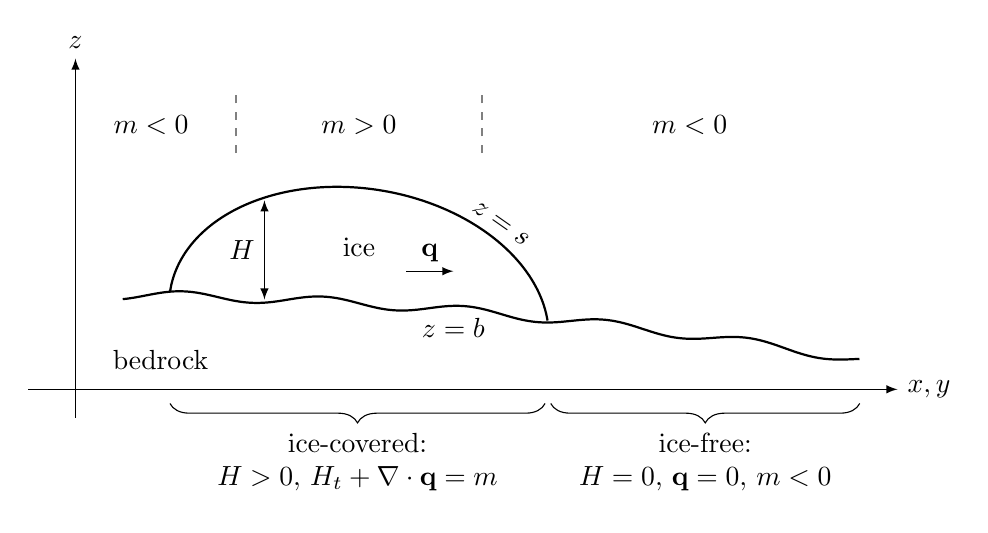
\begin{tikzpicture}[scale=1.2,
declare function={ bed(\x) = 1.0 - 0.01*\x*\x - 0.05*sin(240.0*\x);
                   ice(\x) = 0.7 * sqrt((\x-0.99)*(5.01-\x)) + bed(1.0) - (bed(5.0)-bed(1.0)) * (5.0-\x)/4.0; }]

  % draw axes
  \draw[-latex] (-0.5,0.0) -- (8.7,0.0) node[xshift=4mm] {$x,y$};
  \draw[-latex] (0.0,-0.3) -- (0.0,3.5) node[yshift=2mm] {$z$};

  % bed
  \draw[domain=0.5:8.3,samples=201,variable=\x,black,thick] plot ({\x},{bed(\x)});
  \node at (0.9,0.31) {bedrock};

  % ice surface
  \draw[domain=1.0:5.0,samples=301,variable=\x,black,thick] plot ({\x},{ice(\x)-0.47});  % down-shift needed to fix; WHY?

  % labels/arrows on or within ice
  \node at (3.0,1.5) {ice};
  \node[rotate=-35] at (4.5,1.75) {$z=s$};
  \node at (4.0,0.65) {$z=b$};
  \draw[-latex] (3.5,1.25) -- (4.0,1.25) node[midway,above] {$\mathbf{q}$};
  \draw[latex-latex] (2.0,0.95) -- (2.0,2.0) node[midway,left] {$H$};

  % labels and dashed lines showing CMB zones
  \node at (0.8,2.8) {$m<0$};
  \draw[dashed,thick,gray] (1.7,2.5) -- (1.7,3.2);
  \node at (3.0,2.8) {$m>0$};
  \draw[dashed,thick,gray] (4.3,2.5) -- (4.3,3.2);
  \node at (6.5,2.8) {$m<0$};

  % underbraces with labels
  \draw[decorate,decoration={brace,amplitude=7pt,mirror}] (1.0,-0.15) -- (4.97,-0.15) node[below,midway,yshift=-2mm] {$\begin{matrix} \text{ice-covered:} \\ H>0, \, H_t+\nabla\cdot\mathbf{q}=m \end{matrix}$};
  \draw[decorate,decoration={brace,amplitude=7pt,mirror}] (5.03,-0.15) -- (8.3,-0.15) node[below,midway,yshift=-2mm] {$\begin{matrix} \text{ice-free:} \\ H=0, \, \mathbf{q}=0, \, m < 0 \end{matrix}$};

\end{tikzpicture}


\end{center}
\caption{An ice sheet with adjacent ice-free areas.}
\label{fig:co:iceschematic}
\end{figure}

\medskip
The mass of ice in any region $V\subseteq \Omega$ is $\int_V \rho H$, where $\rho$ is the (constant) density of ice in $\text{kg} \, \text{m}^{-3}$.  To describe how this mass changes by flow through $\partial V$ we use a flux $\hat{\mathbf{q}}$ with units $\text{kg} \,\text{s}^{-1}\,\text{m}^{-1}$.  The mass can also change according to the source term, the CMB $\hat{m}(t,x,y)$ in $\text{kg} \,\text{s}^{-1}\,\text{m}^{-2}$, so mass conservation says
\begin{equation}
\frac{d}{dt}\left(\int_V \rho H\right) = - \int_{\partial V} \hat{\mathbf{q}} \cdot \mathbf{n} + \int_V \hat{m},
\end{equation}
where $\mathbf{n} \in \RR^2$ is the outward unit vector along $\partial V$.  Now divide by $\rho$ and define $\mathbf{q}=\hat{\mathbf{q}}/\rho$ and $m=\hat{m}/\rho$.  Using the divergence (Green's) theorem in the plane then yields the strong form of the mass conservation equation, applying in any open subset of $\Omega \times [0,t_f]$ which is ice-covered:
\begin{equation}
H_t + \Div \mathbf{q} = m \qquad \text{ if } H>0.   \label{eq:co:iceconservation}
\end{equation}

However, a fundamental idea is that if the annual balance of snowfall versus melt is consistently positive at a given location and period of time (e.g.~years) then a glacier is present.  The contrapositive of this statement is that ice-free locations have non-positive CMB \cite{Bueler2016,JouvetBueler2012}, so consider a place where there is no ice, that is, an open subset of $\Omega \times [0,t_f]$ where $H=0$.  Then, because ice flux $\mathbf{q}$ scales with a positive power of ice thickness (below), and thus the flux is also zero at ice-free points, we have
\begin{equation}
H_t = 0 \quad \text{ and } \quad \mathbf{q} = 0 \quad \text{ and } \quad m \le 0 \qquad \text{ if } H=0.  \label{eq:co:icefree}
\end{equation}
Figure \ref{fig:co:iceschematic} shows statements \eqref{eq:co:iceconservation} and \eqref{eq:co:icefree} applying in disjoint areas.

FIXME The two \pSNES types which can handle inequality constraints are \texttt{SNESVINEWTONRSLS} and \texttt{SNESVINEWTONSSLS}, abbreviated \texttt{RSLS} and \texttt{SSLS} from now on.   These types allow \emph{bound} (\emph{box}) constraints given by vectors $\mathbf{X}_l,\mathbf{X}_u \in \RR_+^N$,
\begin{equation}
    \mathbf{X}_l \le \mathbf{u} \le \mathbf{X}_u,  \label{eq:co:boxconstraints}
\end{equation}
where $\RR_+=[-\infty,+\infty]$ denotes the extended real line.  In our discretized obstacle problem there is no upper bound so $\mathbf{X}_u=+\infty=$ \texttt{PETSC\_INFINITY}.  Both \texttt{SNESVI} types are modifications of the line-search Newton method \cite[Chapter 4]{Buelerbook}.  They were originally designed to solve finite-dimensional \emph{nonlinear complementarity problems} (NCPs)
\begin{equation}
       F(\bw) \ge 0 \quad \text{ and } \quad \bw \ge 0 \quad \text{ and } \quad \bw F(\bw) = 0, \label{eq:co:NCP}
\end{equation}
where $\bw \in \RR^N$ \cite{BensonMunson2006}, though they have been enhanced to allow two-sided bounds \eqref{eq:co:boxconstraints}.  The function $F:\RR^N \to \RR^N$ is again called the \emph{residual} in this strong form.  The last condition in \eqref{eq:co:NCP}, \emph{complementarity}, can be interpreted as a pointwise product $\bw F(\bw) = 0$ \emph{or} as an inner product $\bw^\top F(\bw)=0$; the forms are equivalent because of the first two conditions.  In any case, complementarity says that either an entry $w_i$ is zero or that the corresponding residual entry $F_i(\bw)$ is zero.  Note that \emph{nondegeneracy} means that for each $i$ either $w_i$ or $F_i(\bw)$ is positive.

We have arrived at an NCP.  That is, if we write $\Phi(H) = H_t + \Div \mathbf{q} - m$ then
\begin{equation}
\Phi(H) \ge 0, \quad H \ge 0, \quad \text{ and } \quad H\, \Phi(H) = 0  \label{eq:co:iceNCP}
\end{equation}
almost everywhere on $\Omega \times [0,t_f]$.  However, to give a precise meaning to \eqref{eq:co:iceNCP}, it remains to add ice dynamics.  That is, we need a formula which determines flux $\mathbf{q}$ from the boundary stresses and body forces on the ice sheet.  Such formulas arise from two sources: experimentally-derived viscous laws in the small and momentum conservation equations in the large.  For the former we use a power law relating shear stress to deformation rate, namely the Glen flow law for ice \cite{GreveBlatter2009}.  For the latter, conservation of momentum could be described by a separate set of equations, e.g.~the variable-viscosity Stokes equations, but here we use a simpler model.  The shallow ice approximation (SIA) flux is diffusive and computes the flux from the local values of the thickness and the surface elevation gradient \cite{Fowler1997,GreveBlatter2009}:
\begin{equation}
\mathbf{q} = - \Gamma H^{n+2} |\grad s|^{n-1} \grad s. \label{eq:co:iceflux}
\end{equation}
Here $n > 1$ is the \emph{Glen exponent} \cite{GreveBlatter2009} and we collect a constant $\Gamma = 2 A (\rho g)^n / (n+2)>0$.  The \emph{ice softness} $A>0$ is constant because the model is isothermal.

The time-dependent SIA model combines equations \eqref{eq:co:iceconservation} and \eqref{eq:co:iceflux} into an equation for evolution of the ice thickness:
\begin{equation}
H_t - \Div\left( \Gamma H^{n+2} |\grad s|^{n-1} \grad s\right) = m.   \label{eq:co:SIA}
\end{equation}
(This equation can also be regarded as evolving surface elevation, with $s_t=H_t$ because of our assumption that $b_t=0$.  Note $\grad s = \grad H + \grad b$.)  Observe that the second-order nonlinear operator in \eqref{eq:co:SIA} combines features of the $p$-Laplacian \cite{BarrettLiu1993} and porous medium \cite{Vazquez2007} operators.

The applied stresses considered in land-terminating ice flow models include only the body force of gravity and resistance to sliding at the base.  (The stresses applied by the atmosphere are negligible.)  Model \eqref{eq:co:SIA} makes the simple assumption that the sliding velocity is zero because the base of the ice has high resistance, or that the ice is frozen to the bed.  A more complete approximation of the Stokes equations is needed to model actual sliding \cite{BuelerBrown2009}.

There are various ways of identifying the diffusive and transport parts of \eqref{eq:co:SIA}.  Here we define a \emph{diffusivity} and a \emph{pseudo-velocity} \cite{Bueler2016},
\begin{equation}
D = \Gamma H^{n+2} |\grad H + \grad b|^{n-1}, \qquad \mathbf{W} = - \Gamma |\grad H + \grad b|^{n-1} \grad b;  \label{eq:co:DWdefns}
\end{equation}
these are defined for any $H\in W^{1,p}(\Omega)$.  Thus we rewrite \eqref{eq:co:SIA} as a kind of formal diffusion-advection-reaction equation for the ice thickness evolution
\begin{equation}
H_t - \Div\left(D \grad H\right) + \Div\left(\bW H^{n+2}\right) = m.   \label{eq:co:SIAdar}
\end{equation}
The diffusivity $D \ge 0$ has the usual units (e.g.~$\text{m}^2 \,\text{s}^{-1}$) but $\bW$ has units $\text{m}^{-n} \,\text{s}^{-1}$.  Though $\bW$ is not a true velocity it is helpful to think about that term as transport in the direction of $-\grad b$.  When the bed is flat ($\grad b=0$) this term disappears and \eqref{eq:co:SIAdar} is a nonlinear diffusion-reaction equation on the set where $H>0$.

We will, however, only solve the steady-state problem.  Suppose $b=b(x,y)\in C^1(\Omega)$.  Also suppose that the CMB $m=m(x,y)$ is both $t$ and $H$ independent and that $m \in C(\Omega)$.  (Our scheme will use point values of $\grad b$ and $m$.)  At locations where $H>0$ we solve the equation
\begin{equation}
- \Div\left(D \grad H\right) + \Div\left(\bW H^{n+2}\right) = m   \label{eq:co:SIAsteady}
\end{equation}
for $H(x,y)$.  At all points of $\Omega$ the condition $H\ge 0$ applies.

When they are posed as variational inequalities, an incomplete theory of well-posedness applies to \eqref{eq:co:SIAdar} and \eqref{eq:co:SIAsteady}.  The time-dependent and steady-state models are well-posed in the flat bed ($\grad b=0$) case \cite{Calvoetal2003} using a power transformation \cite{Raviart1970}.  Existence has been proven for the steady-state model for general beds \cite{JouvetBueler2012}.  Both steady state and time-dependent flat-bed exact solutions are available for verification purposes \cite{vanderVeen2013}.

The diffusion term disappears when $D\to 0$.  By \eqref{eq:co:DWdefns} this occurs when either $|\grad s|\to 0$ or $H\to 0$.  That is, this ``doubly-nonlinear'' diffusion degenerates in the manner exhibited by \emph{both} the better-known $p$-Laplacian and porous media nonlinear operators.  These degeneracies imply low regularity at surface elevation extrema ($|\grad s|\to 0$) and at ice sheet margins ($H \to 0$).  The latter ice-margin type of regularity loss, where $|\grad H| \to \infty$ along the free boundary, is both more common and has more severe consequences for numerical approximations.  Figure \ref{fig:co:freeboundaryshape} compares the shape of the solutions of the classical obstacle and ice sheet problems.  The above-mentioned power transformation converts the doubly-nonlinear operator in \eqref{eq:co:SIAsteady} into a $p$-Laplacian nonlinearity, resolving the worst degeneracy, but unfortunately this is only a directly-useful approach in the flat-bed case.

\begin{figure}[h]
\begin{center}
FIXME %\includegraphics[width=0.9\textwidth]{figs/FIXME}
\end{center}
\caption{Solutions of the classical obstacle problem (left) and ice sheet problem (right) near a free boundary.}
\label{fig:co:freeboundaryshape}
\end{figure}

Problem \eqref{eq:co:SIAsteady} could equivalently be solved for surface elevation $s(x,y)$, in which case the obstacle would be ``$s\ge b$'' instead of ``$H\ge 0$.''  Because of flow, generally $s$ is more regular than $H$ at inactive points, but on the other hand, as an obstacle $b$ is less smooth than the zero function.

After stating the NCP form of the steady-state SIA equation \eqref{eq:co:SIAsteady} we discretize by exploiting FE and FV ideas.  Then we attack this nonlinear-with-inequality-constraints problem using a Newton method (\pSNESVI) and a structured-grid (\pDMDA).


\section{A steady-state ice sheet solver}

FIXME discretization of \eqref{eq:co:SIAsteady} by a $Q^1$ structured-grid FVE method \cite{Bueler2016,EwingLinLin2002}; Figure \ref{fig:co:mstarstencil}.  The ice thickness solution $H(x,y)$ is nonnegative ($H \ge 0$) for any input CMB or bed topography.  The domain is square $\Omega = (0,L) \times (0,L)$ with periodic boundary conditions.

\begin{figure}[h]
\begin{center}
% M* scheme stencil
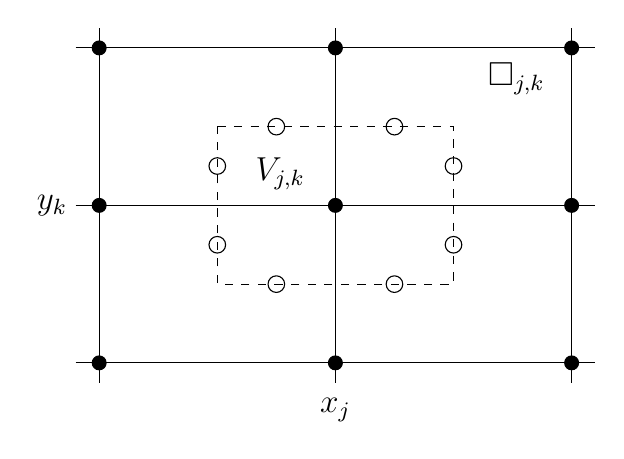
\begin{tikzpicture}[scale=1.0]
  % strong grid around elements beyond 0 and 6 in x and 0 and 4 in y
  \draw (-0.3,0) -- (6.3,0);
  \draw (-0.3,2) -- (6.3,2);
  \draw (-0.3,4) -- (6.3,4);
  \draw (0,-0.25) -- (0,4.25);
  \draw (3,-0.25) -- (3,4.25);
  \draw (6,-0.25) -- (6,4.25);

  % nodes
  \filldraw (0,0) circle (2.5pt);  \filldraw (3,0) circle (2.5pt);  \filldraw (6,0) circle (2.5pt);
  \filldraw (0,2) circle (2.5pt);  \filldraw (3,2) circle (2.5pt);  \filldraw (6,2) circle (2.5pt);
  \filldraw (0,4) circle (2.5pt);  \filldraw (3,4) circle (2.5pt);  \filldraw (6,4) circle (2.5pt);

  % outline control volume
  \draw[dashed] (1.5,3) -- (4.5,3) -- (4.5,1) -- (1.5,1) -- cycle;

  % mark quadrature points
  \draw (4.5,2.5) circle (3.0pt);
  \draw (3.75,3)  circle (3.0pt);
  \draw (2.25,3)  circle (3.0pt);
  \draw (1.5,2.5) circle (3.0pt);
  \draw (1.5,1.5) circle (3.0pt);
  \draw (2.25,1)  circle (3.0pt);
  \draw (3.75,1)  circle (3.0pt);
  \draw (4.5,1.5) circle (3.0pt);

  % label elements and control volume
  \draw (2.3,2.4) node {\large $V_{j,k}$};
  \draw (5.3,3.6) node {\large $\square_{j,k}$};

  % label center point
  \draw (3,-0.6) node {\large $x_j$};
  \draw (-0.6,2) node {\large $y_k$};
\end{tikzpicture}


\end{center}
\caption{The FVE method uses a structured FEM grid of $Q^1$ elements $\square_{j,k}$ (solid) with rectangular control volumes $V_{j,k}$ (dashed).  The discrete scheme computes a flux integral over $\partial V_{j,k}$ using eight quadrature points (circles).}
\label{fig:co:mstarstencil}
\end{figure}

FIXME The program \texttt{ice.c} solves \eqref{eq:co:SIAsteady} as a steady-state nonlinear ice sheet model in 2D.  Requires SNESVI (\texttt{-snes\_type vinewtonrsls|vinewtonssls}) because of the constraint.  Option \texttt{-snes\_fd\_color} works well but is slower by a factor of two or so.



%         References
\bibliography{dnlo}
\bibliographystyle{siam}

%\appendix
%\section{FIXME}   \label{app:FIXME}  FIXME

\end{document}
